\documentclass[a4paper,12pt]{report}
\usepackage{alltt, fancyvrb, url}
\usepackage{graphicx}
\usepackage[export]{adjustbox}
\usepackage[utf8]{inputenc}
\usepackage{float}
\usepackage{hyperref}
\usepackage{minted}
\usepackage{lineno}
\usepackage{array}
\usepackage{tabularray}
\usepackage{pdfpages}
% Questo commentalo se vuoi scrivere in inglese.
\usepackage[italian]{babel}
\graphicspath{{./images/}}

\usepackage[italian]{cleveref}
\title{Relazione dell'elaborato di Basi di Dati
    \\ Sistema di gestione penitenziario}

\author{Leonardo Grimaldi}
\date{\today}   
\begin{document}
\maketitle
\tableofcontents
\chapter{Analisi}
\section{Introduzione}
Viene commissionata da un ente governativo la realizzazione di un software gestionale per una casa circondariale che faciliti il tracciamento di detenuti e loro spostamenti.
\section{Intervista}
\begin{linenumbers}
\modulolinenumbers[5]
Si chiede di realizzare un portale che consenta di gestire e storicizzare varie operazioni comuni di un carcere. Per i \textbf{detenuti} in arrivo si vogliono memorizzare gli estremi della persona.
%
I dati richiesti sono:
\begin{itemize}
    \item Nome, cognome, data di nascita, il numero della carta d'identità, altezza
\end{itemize}
Il carcere gestisce solamente detenuti italiani maggiorenni in possesso di carta d'identità quindi non occorre gestire il caso in cui essa non sia presente.
%
Un detenuto può essere rilasciato e rientrare nel carcere, ma anche decedere durante la sua permanenza.
%
Ai detenuti sono assegnate delle \textbf{celle} \underline{letto} in base alla disponibilità.
%
Esse hanno una capacità e più prigionieri possono risiedere al loro interno.
%
\par
Nel corso della loro permanenza le assegnazioni possono subire variazioni e si dovrà quindi tenere traccia degli \textbf{spostamenti}.
%
Questo include la data e ora di uscita e in quale cella è avvenuto lo spostamento.
%
All'interno della prigione sono presenti anche celle \underline{mediche} e \underline{solitarie} all'interno delle quali il prigioniero può risiedere temporaneamente.
%
Ogni cella appartiene a un \textbf{piano} che viene pattugliato da una o più \underline{guardie}.
%
Ogni piano fa parte di un solo \textbf{blocco}.
%
I \underline{turni di pattuglia} sono assegnati in base a un \textbf{orario} prestabilito in cui ogni giorno della settimana è formato da 3 turni:
\begin{itemize}
    \item Mattina: 06:00 - 14:00
    \item Pomeriggio/sera: 14:00 - 22:00
    \item Notte: 22:00 - 06:00 (del giorno successivo)
\end{itemize}   
La guardia lavorerà quindi per 8 ore al giorno con una pausa intermedia di 30 minuti e fine turno di 30 minuti.
%
Le pause e i cambi di turno non verranno gestiti dal database ai fini di copertura dell'orario, ma si suppone che vi sia una guardia di riserva che subentra temporaneamente.
%
\par Il \textbf{personale} del carcere è formato quindi da guardie, ma anche da \underline{amministratori} e di entrambi si vuole memorizzare: il nome, cognome, data di nascita, sesso e codice fiscale.
%
Gli amministratori sono le persone che hanno accesso al sistema gestionale e possono essere anche le guardie stesse.
%
Dovranno poter accedere al sistema con una password a loro assegnata.
%
Sia le guardie che gli amministratori possiedono un badge che li identifica univocamente all'interno della struttura.
%
Di loro si vuole memorizzare inoltre:
\begin{itemize}
    \item Nome, cognome, codice fiscale e sesso.
\end{itemize}
\end{linenumbers}
\section{Estrazione dei concetti principali}
Dall'intervista si possono estrapolare diverse figure che consentiranno di modellare lo schema concettuale.
\subsection*{Detenuto}
Sinonimi: prigioniero, carcerato
%
\\Persona rinchiusa nel carcere.
%
Ha una cella letto assegnata per tutta la permanenza.
%
\subsubsection*{Operazioni}
\begin{itemize}
    \item Trasferimento cella letto
    \item Spostamento temporaneo in celle mediche o solitarie
    \item Dichiarazione di decesso
\end{itemize}
\subsection*{Cella}
In generale, il luogo dove risiede il carcerato.
%
Ha una capacità massima e può essere di tre tipi: letto, medica e solitaria.
%
Può appartenere a un solo piano.
\subsection*{Piano}
Piano dell'edificio. In esso sono contenute molteplici celle.
%
Esso può essere controllato da una o più guardie.
\subsection*{Blocco}
Parte strutturale del carcere dove sono presenti un insieme di piani.
\subsection*{Personale}
L'insieme di persone che non sono detenuti, ma lavorano nel carcere e garantiscono la sicurezza e il suo corretto funzionamento.
%
Si dividono in guardie e amministratori e posseggono un badge.
\subsubsection*{Guardie}
Personale carcerario a cui è affidato il compito di controllare i piani in un certo turno del giorno 
\subsubsection*{Amministratori}
Personale che può accedere al sistema software gestionale attraverso una password.
%
Gli amministratori possono essere anche delle guardie.
\subsubsection*{Operazioni}
\begin{itemize}
    \item Inserimento guardie, assegnazione orario di lavoro
    \item Gestione detenuti: registrazione, trasferimento
\end{itemize}
\subsection*{Orario}
L'orario di lavoro che sarà assegnato alle guardie.
%
Avrà tre turni: mattina (06:00 - 14:00), pomeriggio (14:00 - 22:00) e notte (22:00 - 06:00).
\chapter{Progettazione concettuale}
\section{Schema scheletro}
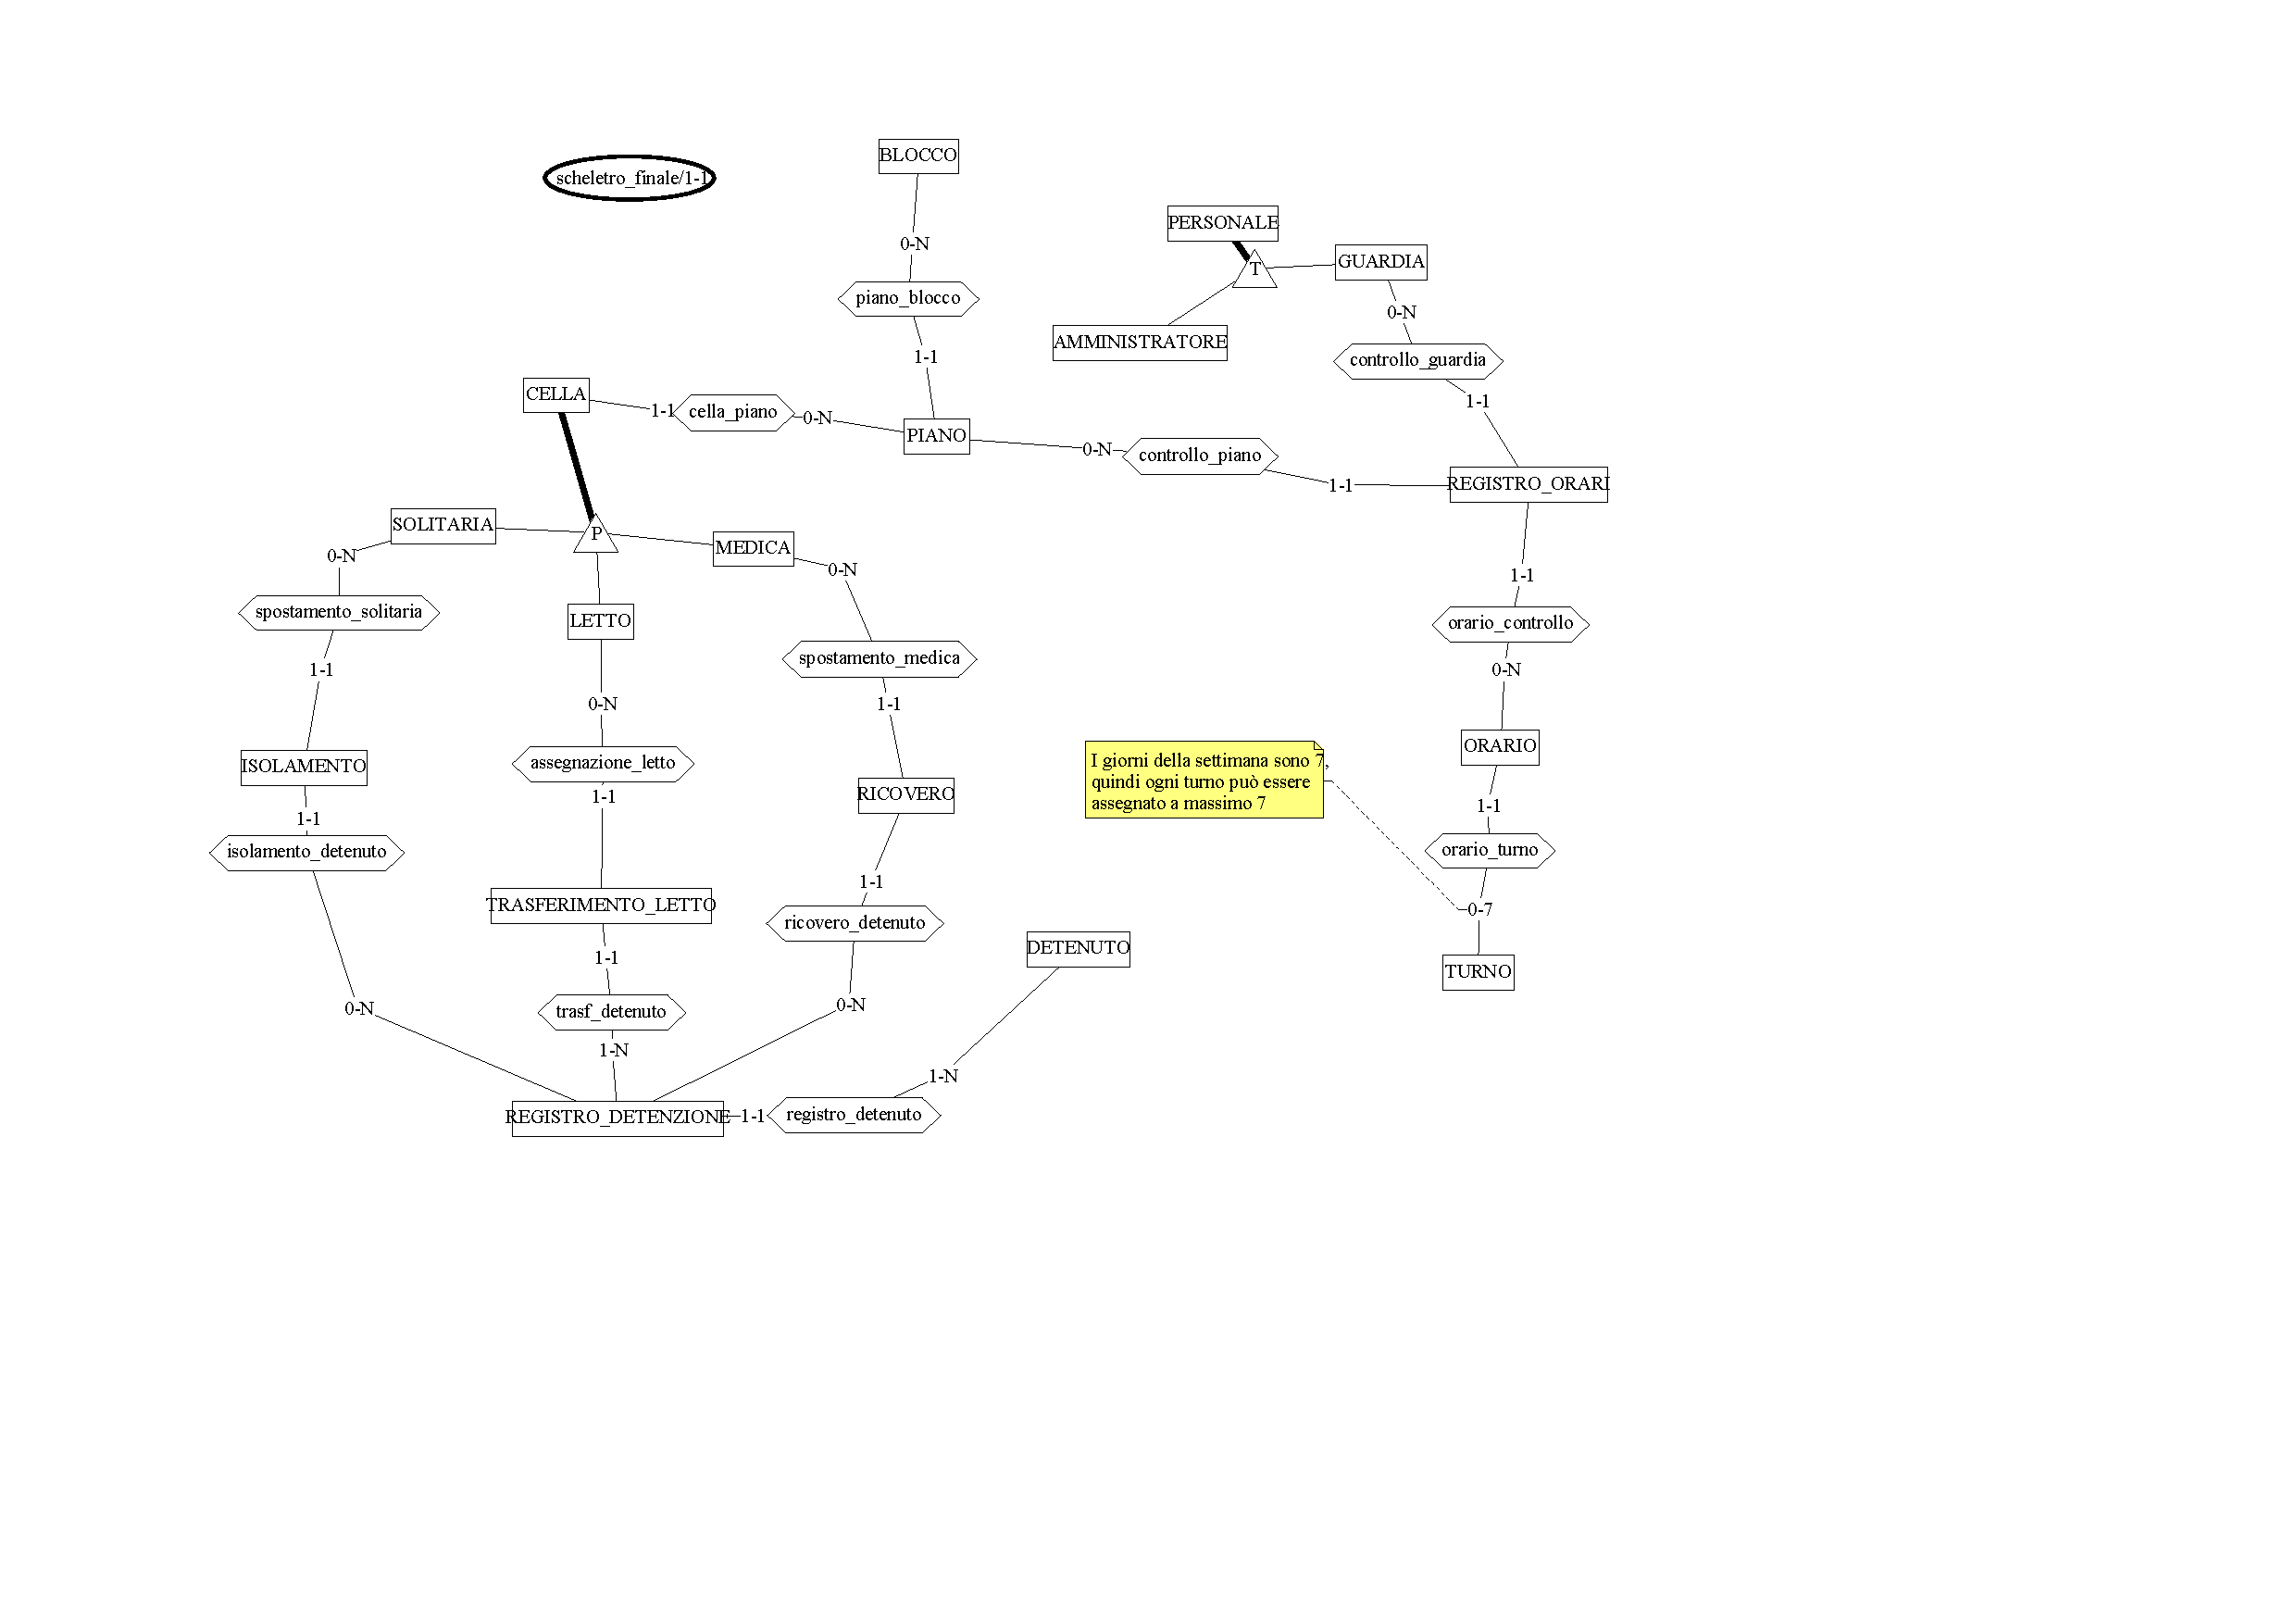
\includepdf[pages={1}, landscape=true, scale=1]{./images/schema_scheletro_finale.pdf}
%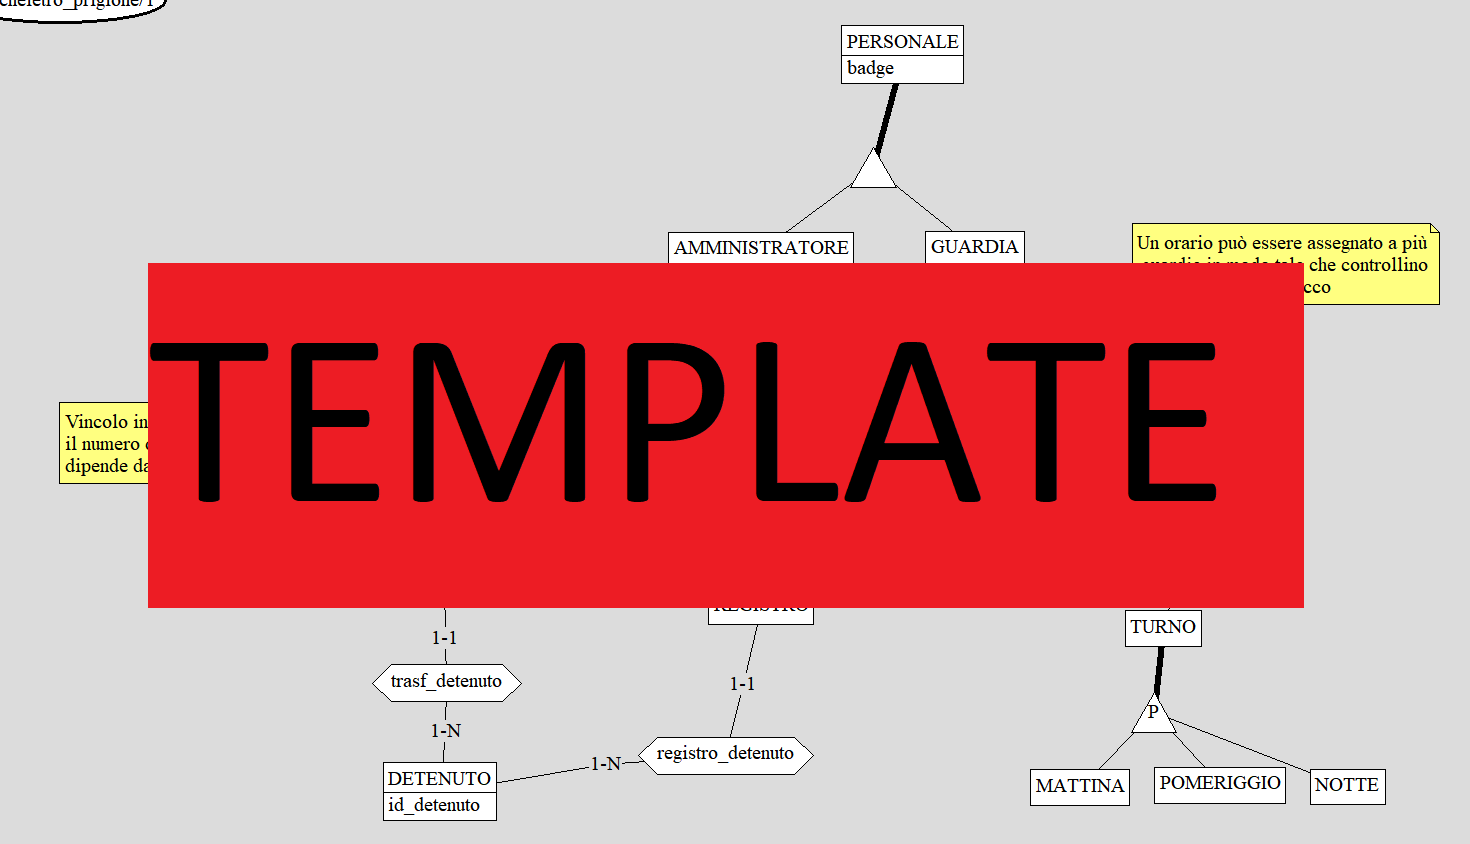
\includegraphics[angle=-90]{er_scheletro_prigione}
\section{Raffinamenti proposti}
Lo schema scheletro è una rappresentazione fedele ai concetti principali estratti nella sezione precedente, ma contiene anche un paio di elementi aggiuntivi che è stato necessario definire per modellare correttamente il dominio.
%
Innanzitutto si possono notare le tre nuove entità TRASFERIMENTO\_LETTO, RICOVERO e ISOLAMENTO che consentiranno di conservare le informazioni sui cambi di celle dei detenuti e ulteriori informazioni come la prognosi oppure il motivo.
%
Tutte queste hanno una cardinalità 1-1 sia dalla parte delle corrispondenti specializzazioni che da quella del REGISTRO\_DETENZIONE (introdotto nel seguente paragrafo) perché un TRASFERIMENTO non può esistere se manca un riferimento a chi e dove è stato spostato.
%
\par
Un'altra aggiunta importante è il concetto di REGISTRO\_DETENUTO; dall'intervista si è analizzato che un prigioniero potrebbe rientrare nel sistema e quindi si è creata la necessità di tenere traccia di questi.
%
Modellando così, un detenuto può essere reinserito nel sistema senza perdere informazioni sui suoi incarceramenti passati.
%
I TURNI, invece, sono in associazione 0-7 con l'ORARIO per esprimere il vincolo sul numero di giorni di una settimana (che infatti sono sette)
%
\par
L'entità REGISTRO\_ORARIO consente di storicizzare gli orari di lavoro delle GUARDIE per un certo PIANO.
%
Le cardinalità delle associazioni riferite a questa entità sono state ideate in modo tale da consentire a più GUARDIE di pattugliare un piano e una GUARDIA avere un solo PIANO da controllare in un ORARIO.
\section{Schema concettuale finale}
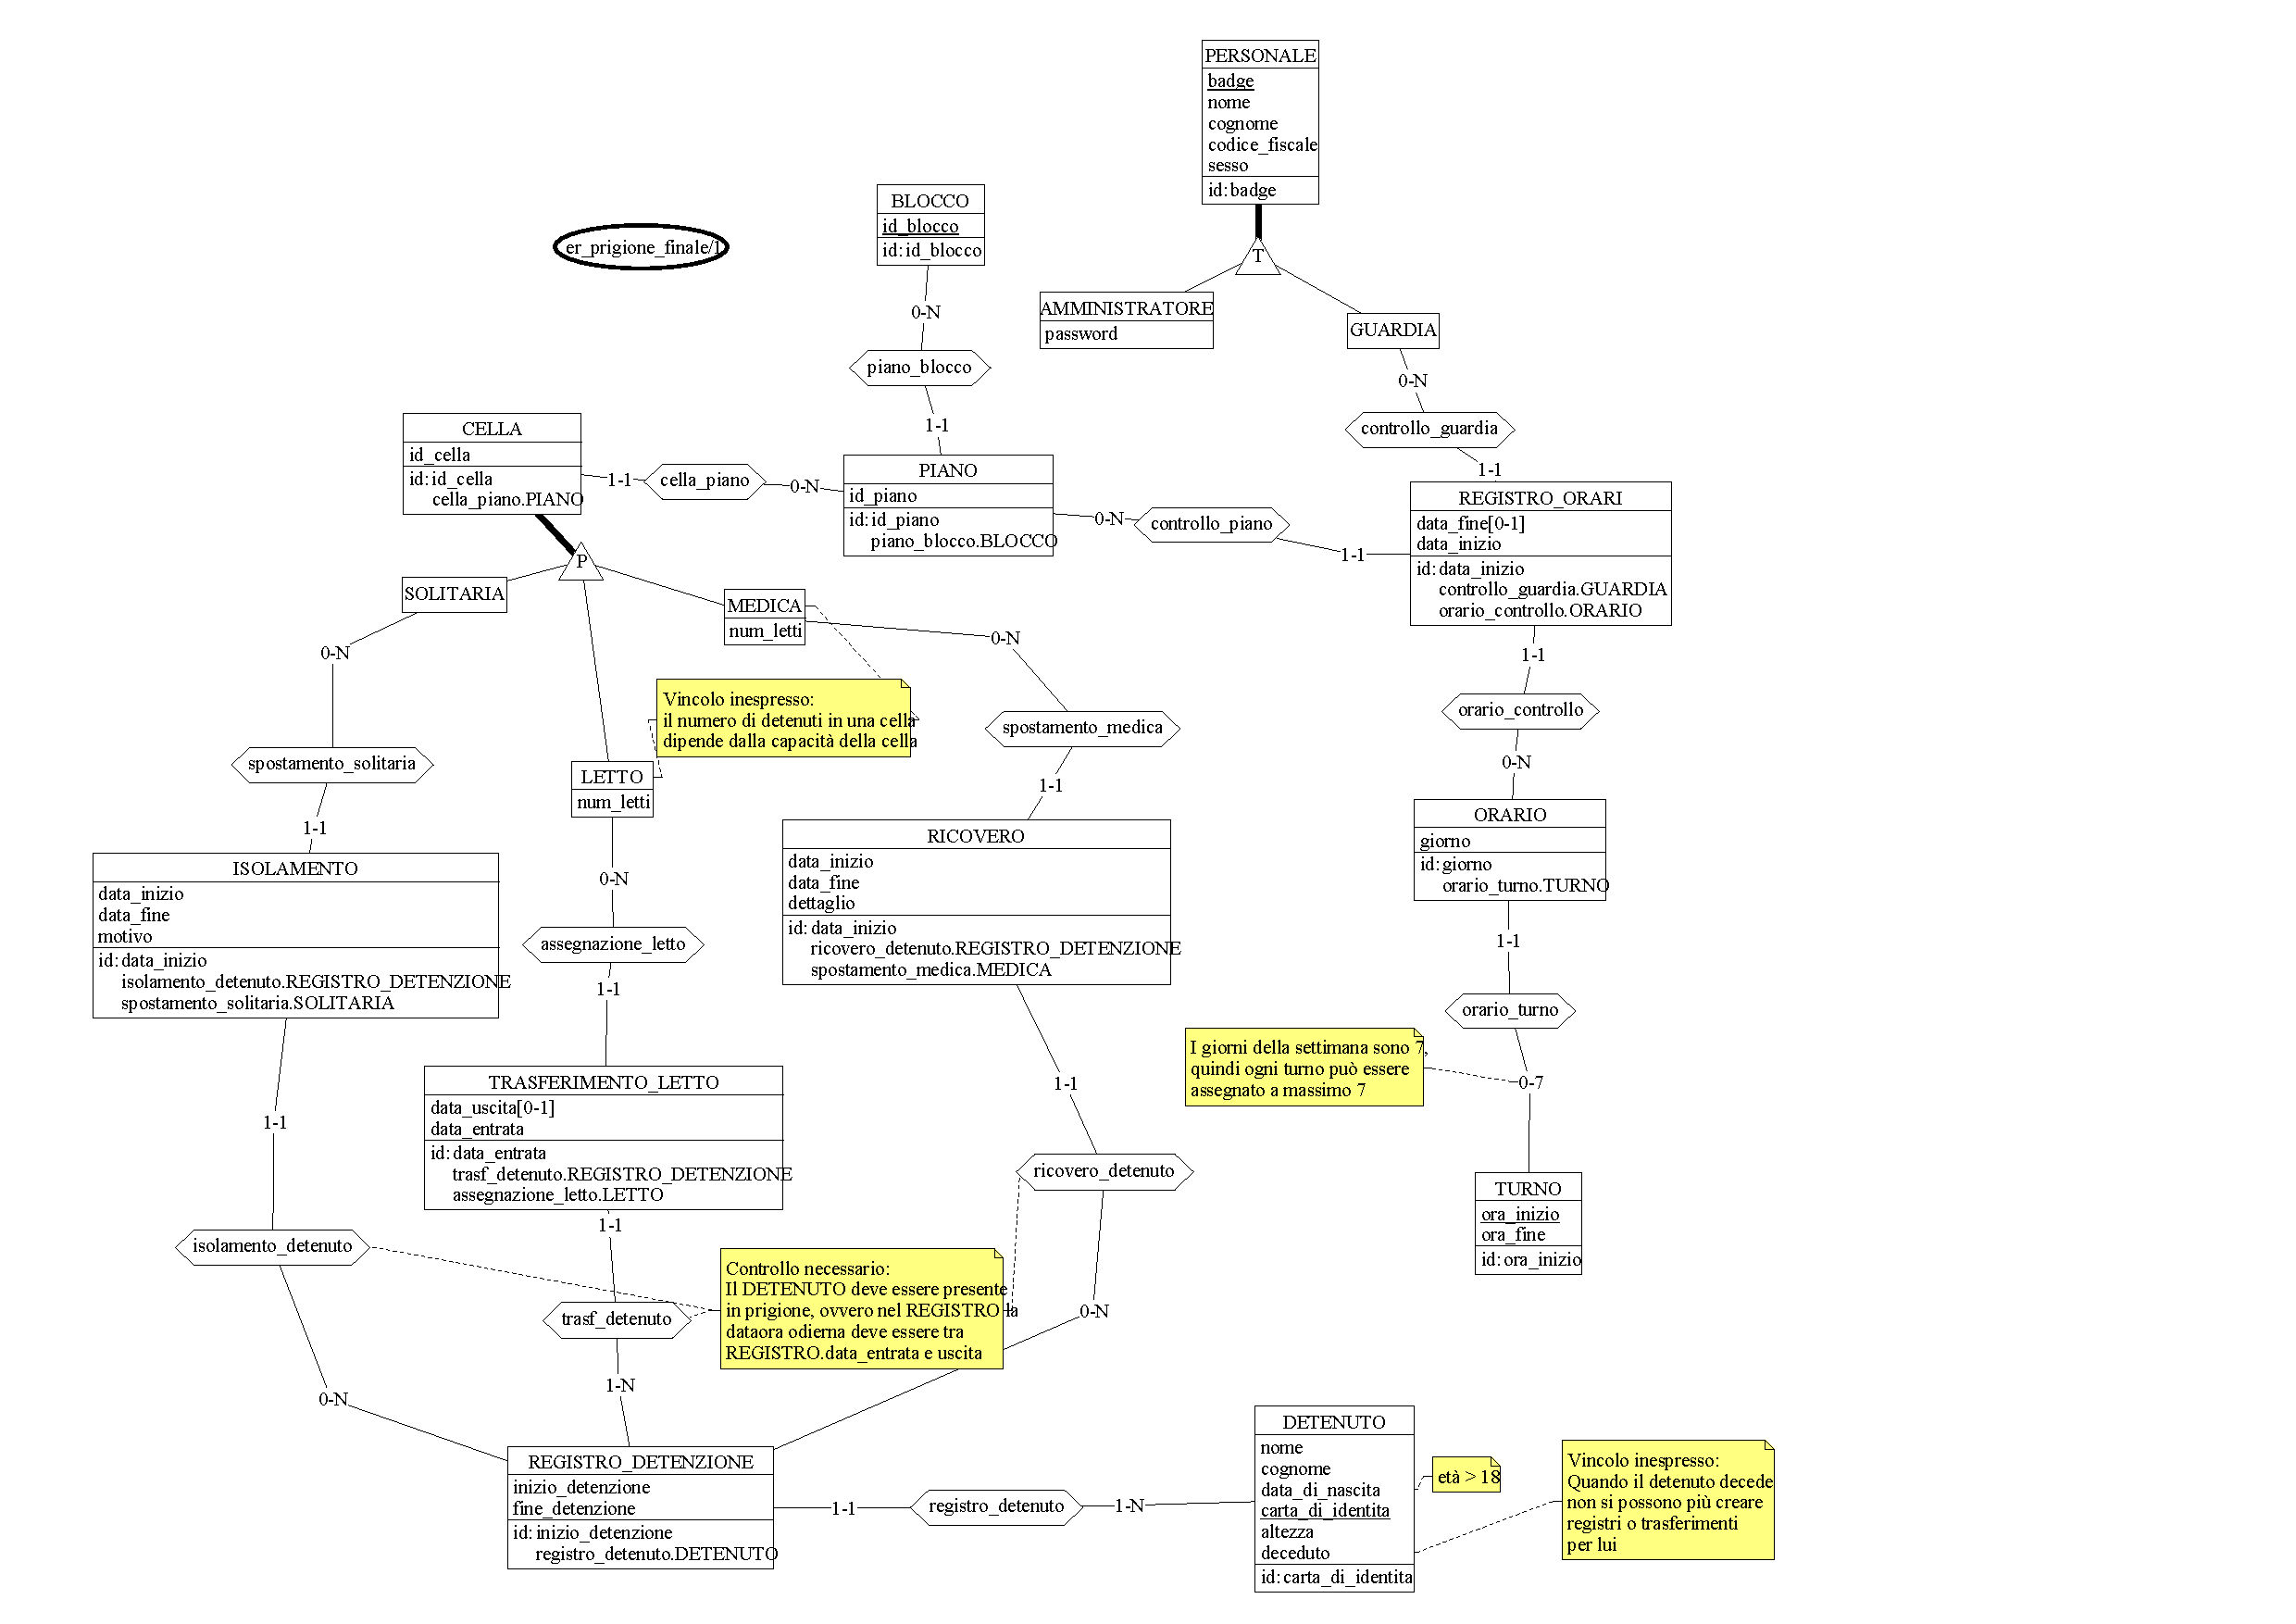
\includepdf[pages={1}, landscape=true, scale=1]{./images/er_finale.pdf}
%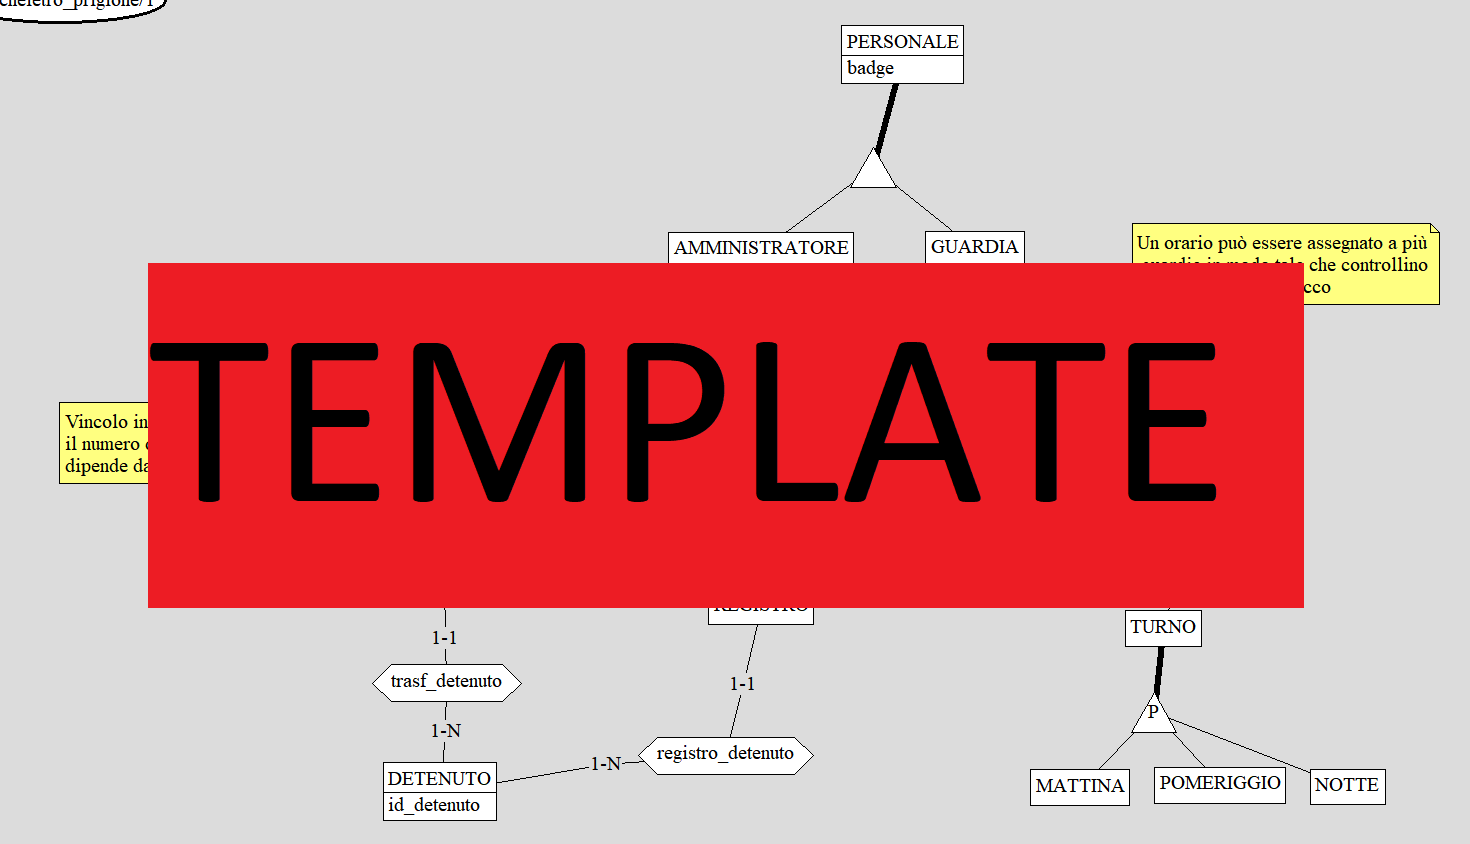
\includegraphics[angle=-90]{er_finale_prigione}
\chapter{Progettazione logica}
\section{Stima del volume dei dati}
Per avere una stima più del volume più precisa si è chiesto al committente la struttura del carcere.
%
La capacità è di 400 persone e vi sono la sezione A e B con due piani e 50 celle ciascuna, abilitate a ospitare massimo due persone.
%
Inoltre, vi è anche la sezione C composta anch'essa da due piani: il primo piano 10 celle solitarie, il secondo 10 celle mediche.
%
\begin{table}[H]
\begin{tabular}{lll}
\hline
Concetto & Costrutto & Volume \\ \hline
DETENUTO & E & 500 \\
assegnazione\_letto & A &  1000 \\
TRASFERIMENTO\_LETTO & E &  1000 \\
trasf\_detenuto & A & 1000 \\
assegnazione\_letto & A & 1000 \\
ISOLAMENTO & E & 200\\
spostamento\_solitaria & A & 200\\
isolamento\_detenuto & A & 200 \\
RICOVERO & E & 350 \\
spostamento\_medica & A & 350 \\
ricovero\_detenuto & A & 350 \\
registro\_detenuto & A & 700 \\
REGISTRO\_DETENZIONE & E & 700 \\
CELLA & E & 220 \\
MEDICA & E & 10\\
LETTO & E & 200 \\
SOLITARIA & E & 10 \\
cella\_piano & A & 220 \\
PIANO & E & 6 \\
piano\_blocco & A & 6 \\
BLOCCO & E & 3 \\
controllo\_piano & A & 175 \\
REGISTRO\_ORARI & E & 175 \\
controllo\_guardia & A & 175 \\
GUARDIA & E & 25 \\
AMMINISTRATORE & E & 10 \\
PERSONALE & E & 35 \\
orario\_controllo & A & 175 \\
ORARIO & E & 21 \\
orario\_turno & A & 21 \\
TURNO & E & 3 \\
\end{tabular}
\end{table}
\section{Descrizione delle operazioni principali e stima della loro frequenza}
\begin{table}[H]
\begin{tabular}{p{9cm} p{2cm} p{1cm}}
\hline
Operazione & Frequenza & Tipo \\ \hline
Inserimento nuovo detenuto & 2/giorno & I \\
Scambio posto letto con un altro detenuto & 5/mese & I \\
Ricoverare un detenuto & 5/mese & I \\
Isolare un detenuto & 3/mese & I \\
Inserimento nuova guardia & 5/anno & I \\
Inserimento nuovo amministratore & 2/anno & I \\
Visualizzare il personale (amministratori, guardie) & 20/giorno & B\\
Visualizzare la lista dei detenuti presenti & 50/giorno & B\\
Visualizzare l'andamento settimanale di nuovi detenuti & 60/giorno & B \\
Visualizzare i primi cinque detenuti che sono stati trasferiti in celle solitarie più volte & 50/mese & B \\
Inserimento nuovo orario & 5/mese & I 
\end{tabular}
\end{table}
\section{Schemi di navigazione e tabelle degli accessi}
In questa parte si elencano le tabelle degli accessi per le operazioni principali e più complesse.
%
Le scritture costano il doppio.
\subsection{Inserire un nuovo detenuto} \label{inserimento}
\begin{enumerate}
    \item Inserire il detenuto
    \item Inserirlo nel registro
    \item Leggere le celle letto libere
        \begin{description}
            \item[Richiede:] Contare i trasferimenti con data uscita NULL per ogni singola cella e verificare che siano minori del numero letti
        \end{description}
    \item Inserirlo in una cella letto
\end{enumerate}
\begin{table}[H]
\begin{tabular}{p{5cm} p{2cm} p{2cm} p{1cm}}
\hline
Concetto & Costrutto & Accessi & Tipo \\ \hline
DETENUTO & E & 1 & S \\
registro\_detenuto & A & 1 & S \\
REGISTRO\_DETENZIONE & E & 1 & S \\
TRASFERIMENTO\_LETTO & E & \(200 * 2 = 400\) & L \\
trasf\_detenuto & A & 1 & S \\
TRASFERIMENTO\_LETTO & E & 1 & S \\
assegnazione\_letto & A & 1 & S \\
\end{tabular}
\end{table}
Nota: \(200 * 2 = 400\) perché 200 sono le celle letto e due sono i posti letto.
%
Costo totale: \((6S * 2 + 400L) * 2/g= 824\)
\newline
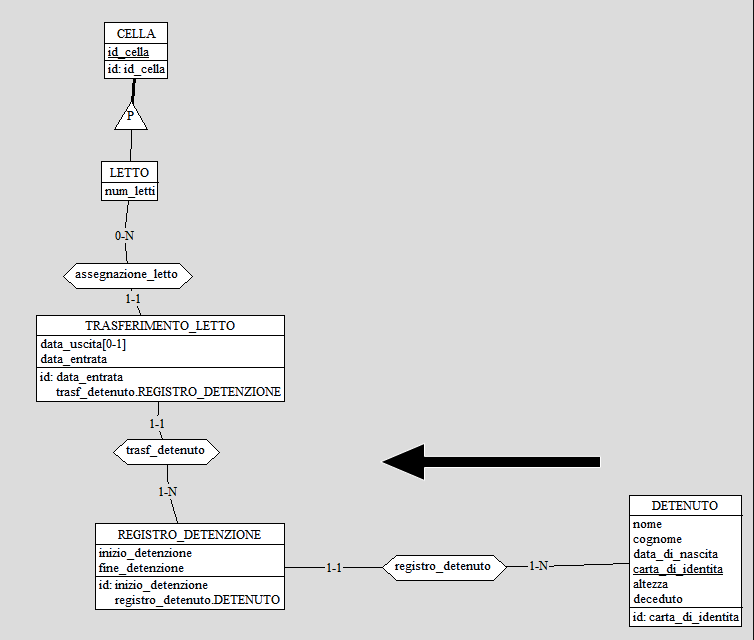
\includegraphics[max size={\textwidth}{\textheight}]{inserire_nuovo_detenuto_con_frecce.png}
\subsection{Scambio posto letto con un altro detenuto}
\begin{itemize}
    \item Visualizzare le celle letto
    \item Visualizzare gli occupanti della cella selezionata
    \item Aggiornare la data uscita del TRASFERIMENTO\_LETTO del primo detenuto
    \item Inserire un nuovo trasferimento per la cella di destinazione
    \item Aggiornare la data uscita del TRASFERIMENTO\_LETTO dell'altro detenuto
    \item Inserire un nuovo trasferimento per l'altro detenuto nella cella del primo
\end{itemize}
\begin{table}[H]
\begin{tabular}{p{5cm} p{2cm} p{1cm} p{1cm}}
\hline
Concetto & Costrutto & Accessi & Tipo \\ \hline
LETTO & E & 200 & L \\
TRASFERIMENTO\_LETTO & E & 2 & L \\
DETENUTO & E & 2 & L \\
trasf\_detenuto & A & 2 & S \\
TRASFERIMENTO\_LETTO & E & 4 & S \\
assegnazione\_letto & A & 2 & S \\
\end{tabular}
\end{table}
Costo totale: \((8S * 2 + 204L) * 5/30g = 36.7\)
\section{Raffinamento dello schema}
\subsection{Specializzazione Amministratore e Guardia}
Per mappare la specializzazione si è deciso di creare una relazione per ogni sottoclasse (in questo caso due) e inserire gli attributi nelle corrispondenti, nonché una chiave esterna che si riferisca alla chiave primaria badge della relazione PERSONALE.
%
Era anche possibile creare una sola relazione PERSONALE con gli attributi delle sotto-entità, ma questo avrebbe portato a maggiori controlli applicativi e valori NULL dato il numero di guardie vs amministratori.
\subsection{Specializzazione Letto, Medica e Solitaria}
Le tre specializzazioni che conferiscono nell'entità CELLA sono totali ed esclusive.
%
Si possono quindi eliminare e creare una unica relazione CELLA che avrà tutti gli attributi delle sottoclassi eliminate: in questo caso solo num\_letti.
%
Viene inoltre aggiunto l'attributo "tipo" che potrà avere come valori ENUM: "Solitaria", "Letto", "Medica" per poter differenziare le singole celle.
%
Sarebbe stato anche possibile eliminare l'entità CELLA e creare tre relazioni, ma così facendo bisognava creare altre tre nuove relazioni da collegare con l'entità PIANO il che avrebbe complicato di molto le query SQL.
%
Facendo in questo modo si ha una unico collegamento con l'entità PIANO, con l'unico svantaggio quello di dover esprimere a livello applicativo vincoli sul tipo.
\subsection{Scelta delle chiavi primarie}
Le chiavi di ogni entità sono già state scelte ed evidenziate nello schema E/R.
%
Per la chiave primaria "badge" di PERSONALE si è fatto riferimento all'intervista del committente nel quale ha espressamente indicato che il personale è in possesso di un codice univoco.
\section{Analisi delle ridondanze}
Data la complessità e il costo delle operazioni di inserimento di un detenuto nonché l'assegnazione di una cella, si è deciso di inserire l'attributo ridondante "posti\_occupati" che verrà incrementato e decrementato quando un detenuto rispettivamente entra o lascia una cella.
%
Ovviamente, questo numero non dovrà mai superare il limite massimo dato da num\_letti, quindi si dovrà gestire questo vincolo a livello applicativo.
%
Dopo l'aggiunta dell'attributo ridondante, la tabella della sezione \ref{inserimento}~\nameref{inserimento} diventerà: 
\begin{table}[H]
\begin{tabular}{p{6cm} p{2cm} p{1cm} p{1cm}}
\hline
Concetto & Costrutto & Accessi & Tipo \\ \hline
DETENUTO & E & 1 & S \\
registro\_detenuto & A & 1 & S \\
REGISTRO\_DETENZIONE & E & 1 & S \\
trasf\_detenuto & A & 1 & S \\
TRASFERIMENTO\_LETTO & E & 1 & S \\
assegnazione\_letto & A & 1 & S \\
CELLA & E & 200 & L \\
TRASFERIMENTO\_LETTO & E & 2 & L \\
CELLA & E & 1 & S
\end{tabular}
\end{table}
Come si può notare, si aggiungono due letture di TRASFERIMENTO\_LETTO per contare i nuovi occupanti e poi si aggiunge una scrittura a CELLA (in precedenza LETTO) per aggiornare l'attributo "posti\_occupati".
\\
Si semplificano così anche le operazione d'isolamento di un detenuto e ricovero che non necessitano la lettura di tutti i record ISOLAMENTO e RICOVERO corrispondenti.
\section{Traduzione di entità e associazioni in relazioni}
detenuto(\underline{carta\_di\_identita}, nome, cognome, data\_di\_nascita, altezza, deceduto)
\\
registro\_detenzione(\underline{inizio\_detenzione}, fine\_detenzione, \underline{carta\_di\_identita: detenuto})
\\
trasferimento\_letto(\underline{data\_entrata}, data\_uscita*, \underline{inizio\_detenzione: registro\_detenzione}, \underline{id\_blocco: cella}, \underline{id\_piano: cella}, \underline{id\_cella: cella})
\\
isolamento(\underline{data\_inizio}, data\_fine, \underline{inizio\_detenzione: registro\_detenzione}, \underline{id\_blocco: cella}, \underline{id\_piano: cella}, \underline{id\_cella: cella}, motivo)
\\
ricovero(\underline{data\_inizio}, data\_fine, \underline{inizio\_detenzione: registro\_detenzione}, \underline{id\_blocco: cella}, \underline{id\_piano: cella}, \underline{id\_cella: cella}, dettaglio)
\\
cella(\underline{id\_blocco: piano}, \underline{id\_piano: piano}, \underline{id\_cella}, tipo, num\_letti, posti\_occupati)
\\
piano(\underline{id\_piano}, \underline{id\_blocco: blocco})
\\
blocco(\underline{id\_blocco})
\\
personale(\underline{badge}, nome, cognome, codice\_fiscale, sesso)
\\
amministratore(\underline{badge: personale}, password)
\\
guardia(\underline{badge: personale})
\\
registro\_orari(\underline{data\_inizio}, \underline{badge: guardia}, \underline{giorno: orario}, data\_fine*)
\\
orario(\underline{giorno}, \underline{ora\_inizio: turno})
\\
turno(\underline{ora\_inizio}, ora\_fine)
\section{Schema relazionale finale}
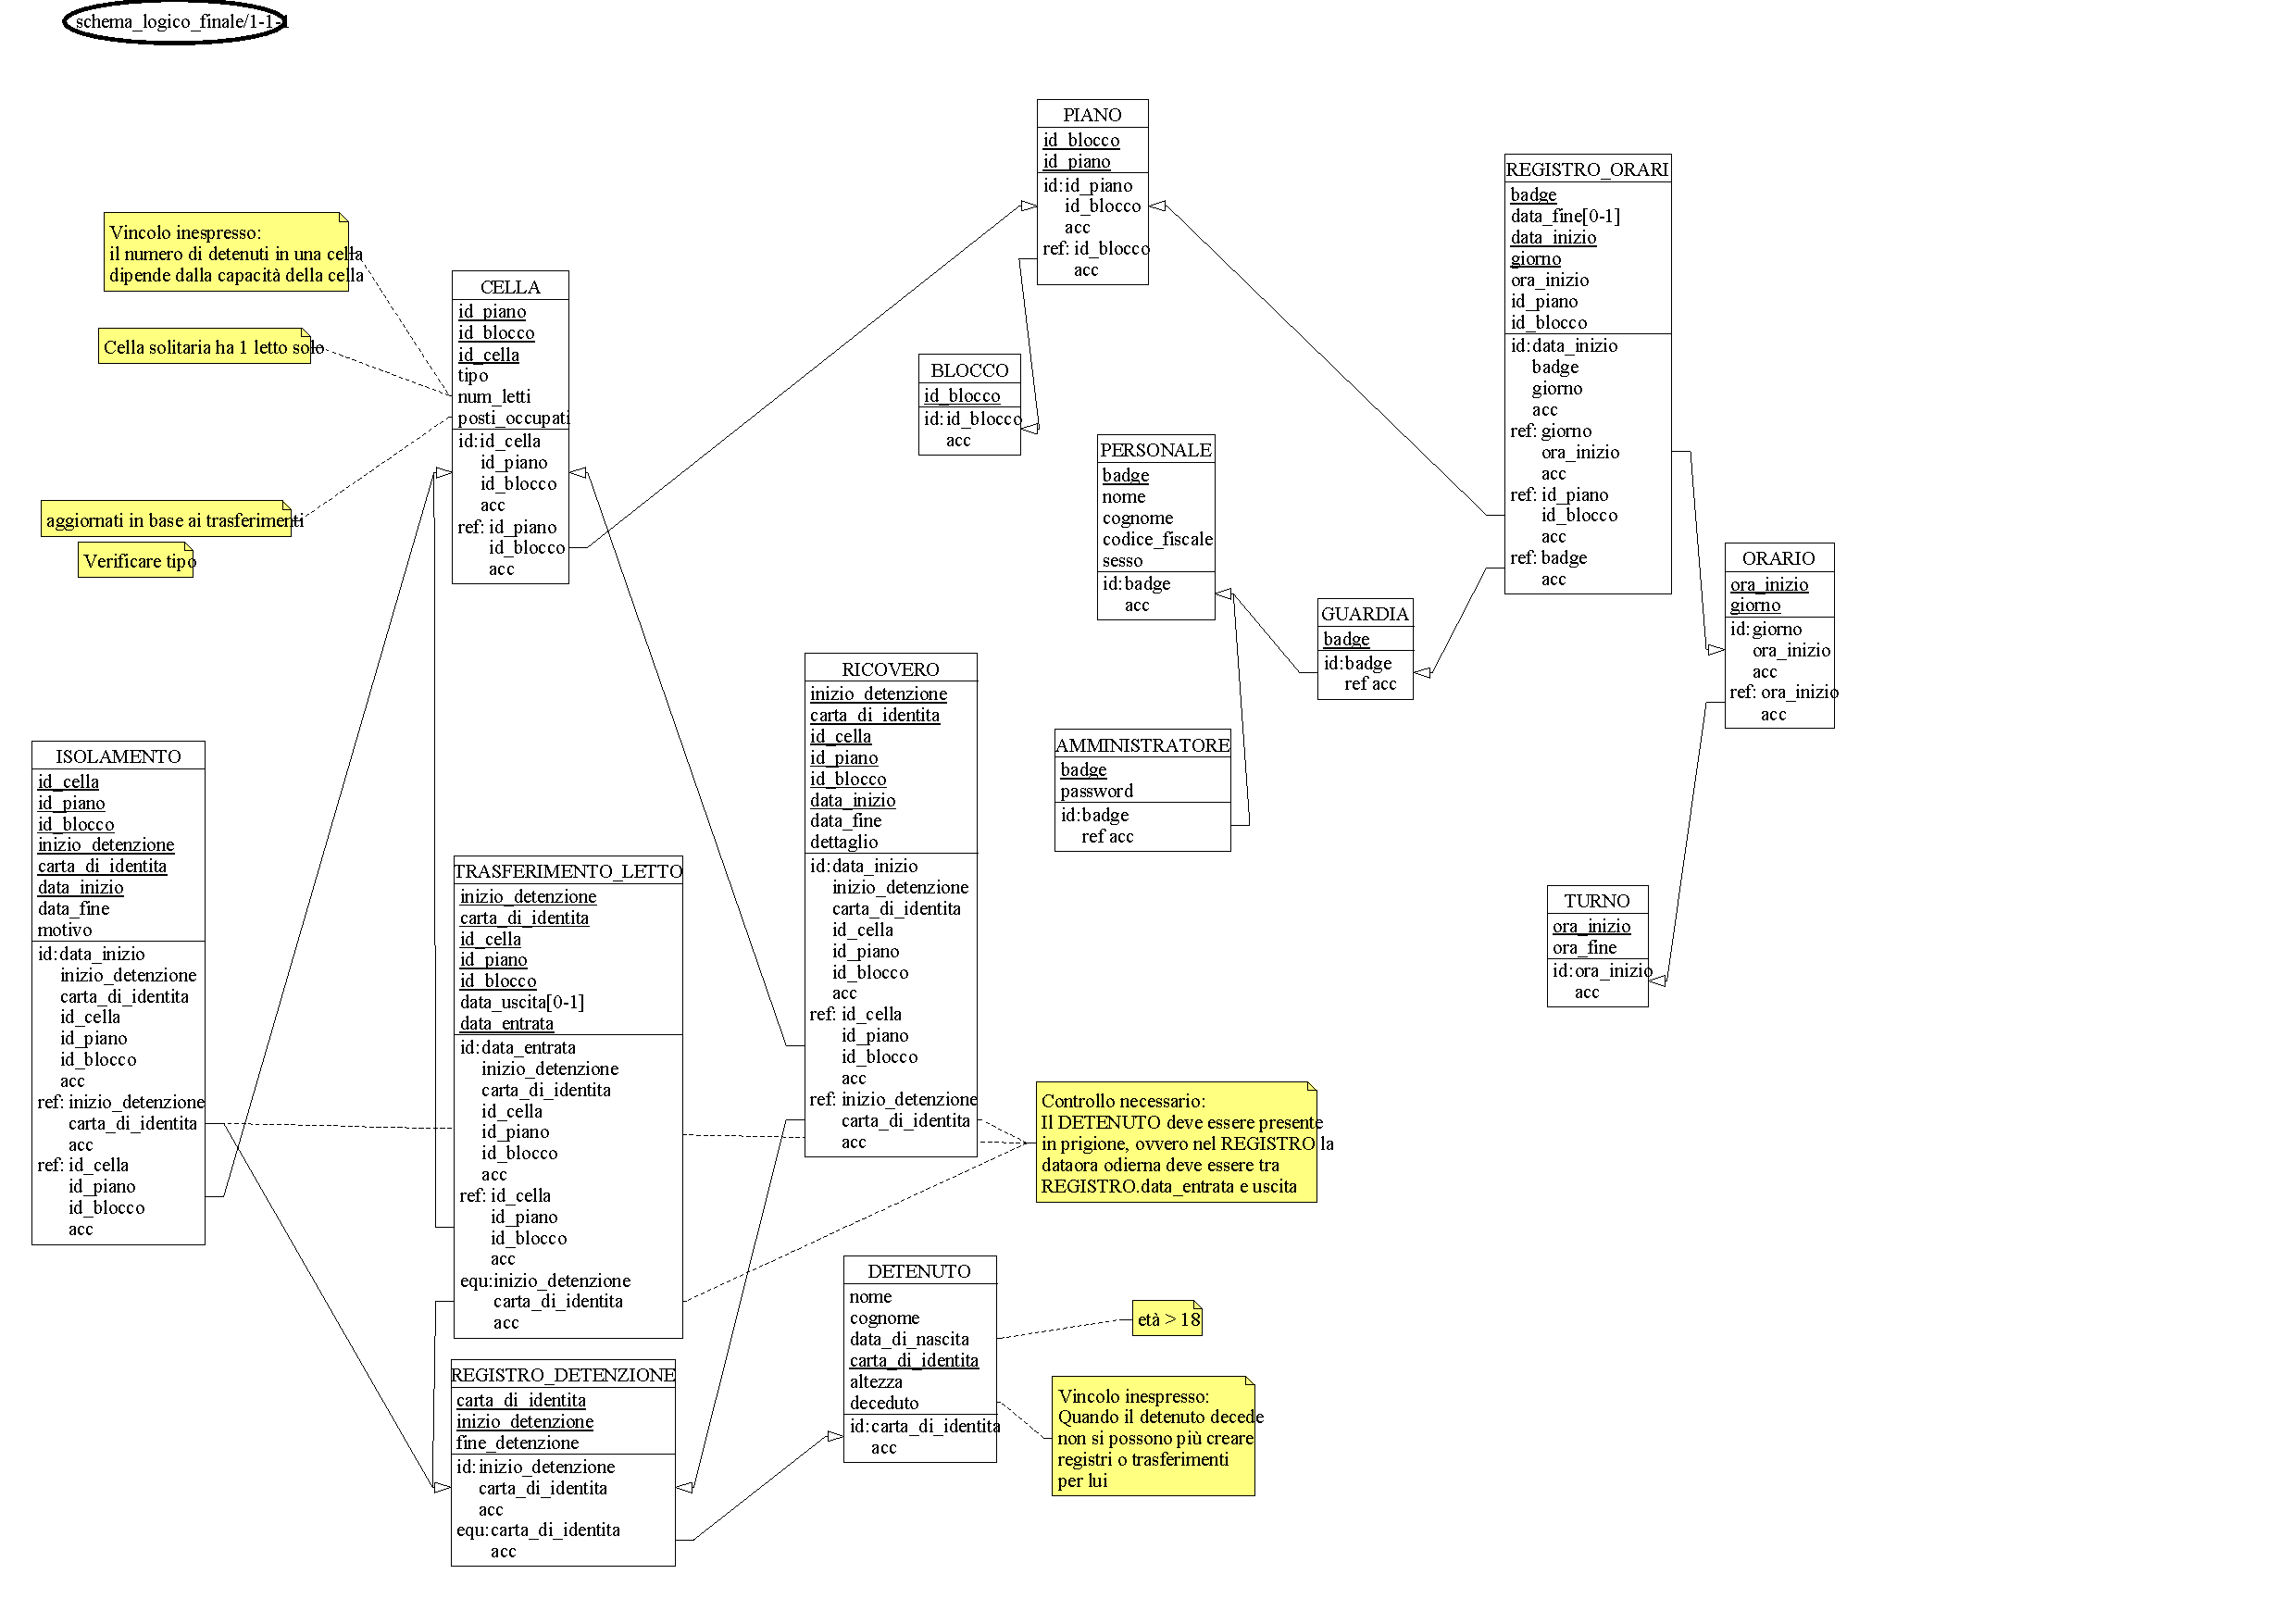
\includepdf[pages={1}, landscape=true, scale=1]{./images/schema_logico_finale.pdf}
\section{Traduzione delle operazioni in query SQL}
\subsection{Inserimento nuovo detenuto}
\begin{minted}[linenos, breaklines]{sql}
INSERT INTO detenuto (nome, cognome, data_di_nascita, carta_di_identita, altezza)
VALUES ($1, $2, $3, $4, $5);
INSERT INTO registro_detenzione (carta_di_identita, inizio_detenzione, fine_detenzione)
VALUES ($1, $2, $3);
INSERT INTO trasferimento_letto (data_entrata, id_blocco, id_piano, id_cella, inizio_detenzione, carta_di_identita)
VALUES ($1, $2, $3, $4, $5, $6);
\end{minted}
Aggiornare i posti occupati
\begin{minted}[linenos, firstnumber=last, breaklines]{sql}
SELECT COUNT(data_entrata) as occupanti
FROM trasferimento_letto
WHERE id_blocco = $1 AND id_piano = $2 AND id_cella = $3 AND data_uscita IS NULL;

UPDATE cella
SET posti_occupati = $1
WHERE id_blocco = $2 AND id_piano = $3 AND id_cella = $4;
\end{minted}
\subsection{Scambio posto letto con un altro detenuto}
\begin{minted}[linenos, breaklines]{sql}
-- Imposto la data uscita a ora
UPDATE trasferimento_letto t
SET data_uscita = NOW()
WHERE t.carta_di_identita = $1 AND data_uscita IS NULL;

INSERT INTO trasferimento_letto (data_entrata, id_blocco, id_piano, id_cella, inizio_detenzione, carta_di_identita)
VALUES (NOW(), $1, $2, $3, (SELECT inizio_detenzione
FROM registro_detenzione r
WHERE r.carta_di_identita = $4
ORDER BY r.inizio_detenzione DESC LIMIT 1), $4);
-- Aggiorno i posti occupati
SELECT COUNT(data_entrata) as occupanti
FROM trasferimento_letto
WHERE id_blocco = $1 AND id_piano = $2 AND id_cella = $3 AND data_uscita IS NULL;

UPDATE cella
SET posti_occupati = $1
WHERE id_blocco = $2 AND id_piano = $3 AND id_cella = $4;
\end{minted}
\subsection{Ricoverare un detenuto}
\begin{minted}[linenos, breaklines]{sql}
INSERT INTO ricovero (id_blocco, id_piano, id_cella, inizio_detenzione, carta_di_identita, data_inizio, data_fine, dettaglio)
VALUES($1, $2, $3, $4, $5, NOW(), $6, $7);
-- Conto i posti occupati
SELECT COUNT(data_inizio) as occupanti
FROM medica
WHERE id_blocco = $1 AND id_piano = $2 AND id_cella = $3 AND NOW() BETWEEN data_inizio AND data_fine;

UPDATE cella
SET posti_occupati = $1
WHERE id_blocco = $2 AND id_piano = $3 AND id_cella = $4;
\end{minted}
\subsection{Isolare un detenuto}
\begin{minted}[linenos, breaklines]{sql}
INSERT INTO isolamento (id_blocco, id_piano, id_cella, inizio_detenzione, carta_di_identita, data_inizio, data_fine, motivo)
VALUES($1, $2, $3, $4, $5, NOW(), $6, $7)
-- Conto i posti occupati
SELECT COUNT(data_inizio) as occupanti
FROM isolamento
WHERE id_blocco = $1 AND id_piano = $2 AND id_cella = $3 AND NOW() BETWEEN data_inizio AND data_fine;

UPDATE cella
SET posti_occupati = $1
WHERE id_blocco = $2 AND id_piano = $3 AND id_cella = $4;
\end{minted}
\subsection{Inserimento nuova guardia}
\begin{minted}[linenos, breaklines]{sql}
INSERT INTO personale (badge, nome, cognome, codice_fiscale, sesso)
VALUES ($1, $2, $3, $4, $5);
INSERT INTO guardia (badge)
VALUES ($1);
\end{minted}
\subsection{Inserimento nuovo amministratore}
\begin{minted}[linenos, breaklines]{sql}
INSERT INTO personale (badge, nome, cognome, codice_fiscale, sesso)
VALUES ($1, $2, $3, $4, $5);
INSERT INTO amministratore (badge, password)
VALUES ($1, $2);
\end{minted}
\subsection{Visualizzare il personale (amministratori, guardie)}
\begin{minted}[linenos, breaklines]{sql}
 SELECT p.badge as "Badge", p.nome as "Nome", p.cognome as "Cognome", p.codice_fiscale as "Codice fiscale", p.sesso as "Sesso", 
    (SELECT COUNT(*) AS num
    FROM guardia g
    WHERE p.badge = g.badge) AS "Guardia",
    (SELECT COUNT(*) AS num
    FROM amministratore a
    WHERE p.badge = a.badge) AS "Amministratore"
FROM personale p;
\end{minted}
\subsection{Visualizzare la lista dei detenuti presenti}
\begin{minted}[linenos, breaklines]{sql}
SELECT d.carta_di_identita AS "CDI", TRIM(d.nome) AS "Nome", TRIM(d.cognome) as "Cognome", r.inizio_detenzione AS "Inizio", r.fine_detenzione AS "Fine", CONCAT(t.id_blocco, t.id_piano, '-', t.id_cella) AS "Cella"
FROM registro_detenzione r
JOIN detenuto d ON r.carta_di_identita = d.carta_di_identita
JOIN trasferimento_letto t ON r.inizio_detenzione = t.inizio_detenzione AND r.carta_di_identita = t.carta_di_identita
WHERE NOW() BETWEEN r.inizio_detenzione AND r.fine_detenzione AND d.deceduto IS NOT TRUE AND t.data_uscita IS NULL
ORDER BY t.data_entrata DESC;
\end{minted}
\subsection{Visualizzare l'andamento settimanale di nuovi detenuti}
\begin{minted}[linenos, breaklines]{sql}
SELECT inizio_detenzione AS "date", COUNT(carta_di_identita) AS "numero"
FROM registro_detenzione
WHERE inizio_detenzione BETWEEN DATE(NOW()) - 7 AND DATE(NOW())
GROUP BY inizio_detenzione
ORDER BY inizio_detenzione ASC
\end{minted}
\subsection{Visualizzare i primi cinque detenuti che sono stati trasferiti in celle solitarie più volte}
\begin{minted}[linenos, breaklines]{sql}
SELECT d.carta_di_identita AS "CDI", TRIM(d.nome) AS "Nome", TRIM(d.cognome) AS "Cognome", COUNT(i.carta_di_identita) AS num
FROM isolamento i
JOIN detenuto d ON i.carta_di_identita = d.carta_di_identita
GROUP BY i.carta_di_identita
ORDER BY num DESC
LIMIT 5
\end{minted}
\subsection{Inserimento nuovo orario}
\begin{minted}[linenos, breaklines]{sql}
INSERT INTO registro_orari (badge, data_inizio, data_fine, giorno, ora_inizio, id_blocco, id_piano)
VALUES ($1, $2, $3, $4, $5, $6, $7);
\end{minted}
\end{document}